
\documentclass[a4paper, 11pt]{article}
\usepackage[margin=3cm]{geometry}
\usepackage[]{fontenc}
\usepackage[utf8]{inputenc}
\usepackage[italian]{babel}
\usepackage{geometry}
\geometry{a4paper, top=2cm, bottom=3cm, left=1.5cm, right=1.5cm, heightrounded, bindingoffset=5mm}
\usepackage{amsmath}
\usepackage{amssymb}
\usepackage{gensymb}
\usepackage{graphicx}
\usepackage{psfrag,amsmath,amsfonts,verbatim}
\usepackage{xcolor}
\usepackage{color,soul}
\usepackage{fancyhdr}
\usepackage{indentfirst}
\usepackage{graphicx}
\usepackage{newlfont}
\usepackage{amssymb}
\usepackage{amsmath}
\usepackage{latexsym}
\usepackage{amsthm}
%\usepackage{subfigure}
\usepackage{subcaption}
\usepackage{psfrag}
\usepackage{footnote}
\usepackage{graphics}
\usepackage{color}
\usepackage{hyperref}
\usepackage{tikz}


\usetikzlibrary{snakes}
\usetikzlibrary{positioning}
\usetikzlibrary{shapes,arrows}


\tikzstyle{block} = [draw, fill=white, rectangle, 
minimum height=3em, minimum width=6em]
\tikzstyle{sum} = [draw, fill=white, circle, node distance=1cm]
\tikzstyle{input} = [coordinate]
\tikzstyle{output} = [coordinate]
\tikzstyle{pinstyle} = [pin edge={to-,thin,black}]

\newcommand{\courseacronym}{CAT}
\newcommand{\coursename}{Controlli Automatici - T}
\newcommand{\tipology}{B}
\newcommand{\trace}{3}
\newcommand{\projectname}{Controllo di meccanismo non-lineare attuato}
\newcommand{\group}{Q}

%opening
\title{ \vspace{-1in}
	\huge \strut \coursename \strut 
	\\
	\Large  \strut Progetto Tipologia \tipology - Traccia \trace 
	\\
	\Large  \strut \projectname\strut
	\\
	\Large  \strut Gruppo \group\strut
	\vspace{-0.4cm}
}
\author{Gaia Margherita, Taruffi Alice, Finocchiaro Alfio}
\date{Febbraio 2025}

\begin{document}
	
	\maketitle
	\vspace{-0.5cm}
	
	Il progetto riguarda il controllo di una tavola rotante motorizzata dotata di giunto cardanico (con elasticità di  coefficiente $k$), attrito viscoso $b$ e motore elettrico che genera la coppia dei momenti in input ($C_M$). La dinamica del sistema è definita dall'equazione differenziale
	%
	\begin{subequations}\label{eq:system}
		\begin{align}
			J\dot \omega &= \tau(\theta) * C_M - \beta\omega - k\theta \\
			\tau(\theta) &= \frac{cos(\alpha)} {1 - ( sin(\alpha) * cos(\theta) )^2}
		\end{align}
	\end{subequations}
	%
	dove $\theta(t)$ rappresenta l'angolo della tavola e $\omega(t)$ la sua velocità angolare.
	
	
	\section{Espressione del sistema in forma di stato e calcolo del sistema linearizzato intorno ad una coppia di equilibrio}
	
	Innanzitutto, esprimiamo il sistema~\eqref{eq:system} nella seguente forma di stato
	%
	\begin{subequations}
		\begin{align}\label{eq:state_form}
			\dot{x} &= f(x,u)
			\\
			y &= h(x,u).
		\end{align}
	\end{subequations}
	%
	Pertanto, andiamo individuare lo stato $x$, l'ingresso $u$ e l'uscita $y$ del sistema come segue 
	%
	\begin{align*}
		x := \begin{bmatrix}
			\theta \\
			\omega
		\end{bmatrix}, \quad u := C_M, \quad y := \theta.
	\end{align*}
	%
	Coerentemente con questa scelta, ricaviamo dal sistema~\eqref{eq:system} la seguente espressione per le funzioni $f$ ed $h$
	%
	\begin{align*}
		f(x,u) &:= \begin{bmatrix}
			x_2 \\
			\frac{u*\tau(x_1)}{J}-\frac{\beta x_2}{J}-\frac{k x_1}{J}
		\end{bmatrix}
		\\
		h(x,u) &:= x_1.
	\end{align*}
	%
	Una volta calcolate $f$ ed $h$ esprimiamo~\eqref{eq:system} nella seguente forma di stato
	%
	\begin{subequations}\label{eq:our_system_state_form}
		\begin{gather*}
			\begin{bmatrix}
				\dot{x}_1
				\\
				\dot{x_2}
			\end{bmatrix} = \begin{bmatrix}
				x_2 \\
				\frac{u*\tau(x_1)}{J}-\frac{\beta x_2}{J}- \frac{k x_1}{J}
			\end{bmatrix} \label{eq:state_form_1}
			\\ 
			y = x_1.
		\end{gather*}
	\end{subequations}
	%
	Per trovare la coppia di equilibrio $(x_e, u_e)$ di~\eqref{eq:our_system_state_form}, andiamo a risolvere il seguente sistema di equazioni
	%
	\begin{align}
		\begin{cases}
			x_{2e} = 0 \\
			\frac{u_e*\tau(x_{1e})}{J} - \frac{k x_{1e} } {J} &= 0 \implies u_e = \frac{k x_{1e}}{\tau(x_{1e})}
		\end{cases}
	\end{align}
	%
	dal quale otteniamo
	%
	\begin{align}
		x_e := \begin{bmatrix}
			\theta_e \\
			\omega_e
		\end{bmatrix} = \begin{bmatrix}
			\frac{5}{9}\pi \\
			0
		\end{bmatrix},  \quad u_e = 424,5 \pi.\label{eq:equilibirum_pair}
	\end{align}
	%
	Definiamo le variabili alle variazioni $\delta x$, $\delta u$ e $\delta y$ come 
	%
	\begin{align*}
		\delta x &= x(t) - x_e, 
		\quad
		\delta u = u(t) - u_e, 
		\quad
		\delta y = y(t) - y_e.
	\end{align*}
	%
	L'evoluzione del sistema espressa nelle variabili alle variazioni pu\`o essere approssimativamente descritta mediante il seguente sistema lineare
	%
	\begin{subequations}\label{eq:linearized_system}
		\begin{align}
			\delta \dot{x} &= A\delta x + B\delta u
			\\
			\delta y &= C\delta x + D\delta u,
		\end{align}
	\end{subequations}
	%
	dove le matrici $A$, $B$, $C$ e $D$ vengono calcolate come
	%
	\newcommand{\pdv}[2]{\frac{\partial}{\partial #1}#2(x,u)|_{x_e,u_e}}
	\begin{subequations}\label{eq:matrices}
		\begin{align}
			A &=\begin{bmatrix}
				\pdv{x_1}{f_1} & \pdv{x_2}{f_1} \\
				\pdv{x_1}{f_2} & \pdv{x_2}{f_2}
			\end{bmatrix} = \begin{bmatrix}
				0 & 1 \\
				\frac{u_e\tau'(x_{1e})}{J} - \frac{k}{J} & - \frac{\beta}{J}
			\end{bmatrix}
			\\
			B &=\begin{bmatrix}
				\pdv{u}{f_1} \\
				\pdv{u}{f_2}
			\end{bmatrix} = \begin{bmatrix}
				0 \\
				\frac{\tau(x_{1e})}{J}
			\end{bmatrix}
			\\
			C &=\begin{bmatrix}
				\pdv{x_1}{h} & \pdv{x_2}{h}
			\end{bmatrix} = \begin{bmatrix}
				1 & 0
			\end{bmatrix}
			\\
			D &= \begin{bmatrix}
				\pdv{u}{h}
			\end{bmatrix} = \begin{bmatrix}
				0
			\end{bmatrix}
		\end{align}
	\end{subequations}
	dove $\tau'(x_1)= - \frac{2sin^2(\alpha)cos(\alpha)sin(\theta)cos(\theta)} 
	{(1-sin^2(\alpha)cos^2(\theta))^2}$.
	\section{Calcolo Funzione di Trasferimento}
	
	In questa sezione, andiamo a calcolare la funzione di trasferimento $G(s)$ dall'ingresso $\delta u$ all'uscita $\delta y$ mediante la seguente formula 
	%
	%
	\begin{align}\label{eq:transfer_function}
		G(s) = C(sI - A)^{-1}B+D = \frac{0.0016359}{s^2 + 0.00125 s + 1.25}.
	\end{align}
	%
	Dunque il sistema linearizzato~\eqref{eq:linearized_system} è caratterizzato dalla funzione di trasferimento~\eqref{eq:transfer_function} con $2$ poli in $-0.000625 + 1.118033i$. In Figura \ref{fig:G} mostriamo il corrispondente diagramma di Bode. 
	
	\begin{figure}[h]
		\centering
		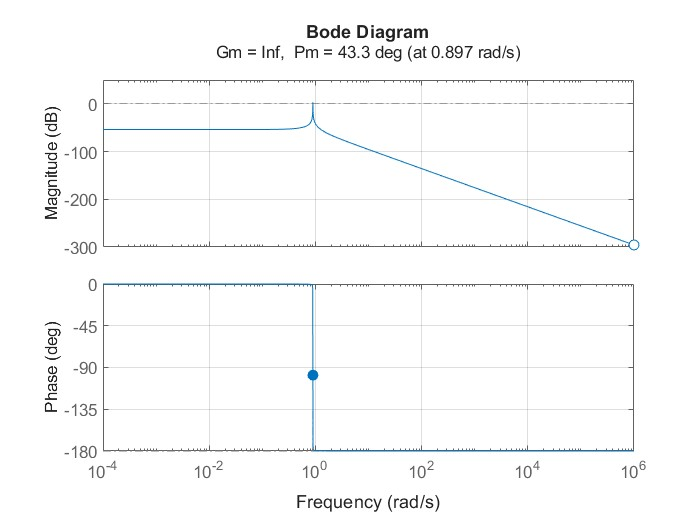
\includegraphics[width=0.5\linewidth]{BodeDiagramWithouthPatch2025.jpg}
		\caption{Diagramma di Bode della $G(s)$.}
		\label{fig:G}
	\end{figure}
	
	\newcommand{\dB}{\text{dB}}
	
	\section{Mappatura specifiche del regolatore}
	\label{sec:specifications}
	
	Le specifiche da soddisfare sono
	\begin{itemize}
		\item[1)] Errore a regime $|e_\infty| \le e_\star = 0.05$ in risposta a un gradino $w(t) = 3(t)$ e $d(t) = 3(t)$
		\item[2)] Per garantire una certa robustezza del sistema si deve avere un margine di fase $M_f \ge 45\degree$.
		\item[3)] Il sistema può accettare una sovraelongazione percentuale al massimo dell’$8\%$ : $S\% \le 8\%$.
		\item[4)]  Il tempo di assestamento alla $\varepsilon\% = 1\%$ deve essere inferiore al valore fissato: $T_{a,\varepsilon} = 0.1s$.
		\item[5)]  Il disturbo sull’uscita $d(t)$, con una banda limitata nel range di pulsazioni $[0, 0.1]$, deve essere abbattuto di almeno 50 dB.
		\item[6)]  Il rumore di misura $n(t)$, con una banda limitata nel range di pulsazioni $[1.5\cdot10^4 , 10^6]$, deve essere
		abbattuto di almeno 60 dB.
	\end{itemize}
	%
	Andiamo ad effettuare la mappatura punto per punto delle specifiche richieste.
	\begin{itemize}
		\item[1)] Per ottenere un errore a regime minore di $e^\star$ in risposta al gradino $w(t) = 3(t)$ con disturbo $d(t) = 3(t)$, avremo un guadagno statico $\mu_s \ge \frac{3 + 3}{e^\star}$ = 120.
		\item[2)] In corrispondenza della pulsazione critica $\omega_c$ si deve avere una fase maggiore di $-135\degree$.
		\item[3)] Per ottenere una sovraelongazione percentuale massima $S\% \le 8\%$ poniamo $\xi = M_f/100.$ Sapendo che la sovraelongazione massima e la $\xi$ massima rispettano la seguente relazione:\[
		S^\star = \exp{\frac{-\pi\xi^\star}{1-(\xi^\star)^2}}
		\]
		Sostituendo $\xi$ otteniamo $M_f = 62.6\degree$.
		\item[4)] Per ottenere un tempo di assestamento al $1\%$ inferiore a $0.1s$ è necessario imporre $e^{-\xi\omega_c T_a} = 0.01$.
		Si ottiene quindi $\xi\omega_c \ge 4.605/T^\star$ con $T^\star$ tempo di assestamento massimo.
		Si ricava quindi $\omega_c=\frac{460.5}{T^\star M_f}=73.49$
		\item[5)] Per riuscire ad attenuare il disturbo in uscita $d(t)$ di 50dB risulta necessario che nell’intervallo
		d’interesse [0; 0.1] $|L(j\omega)|_{\dB} \ge 50\dB$.
		\item[6)] Per riuscire ad attenuare il disturbo di misura $n(t)$ di 50dB risulta necessario che nell’intervallo
		d’interesse $[1.5\cdot10^4 , 10^6]$ $|L(j\omega)|_{\dB} \le -60\dB$.
		
	\end{itemize}  
	
	Pertanto, in Figura \ref{fig:patchedG}, mostriamo il diagramma di Bode della funzione di trasferimento $G(s)$ con le zone proibite emerse dalla mappatura delle specifiche.
	
	\begin{figure}[h!]
		\centering
		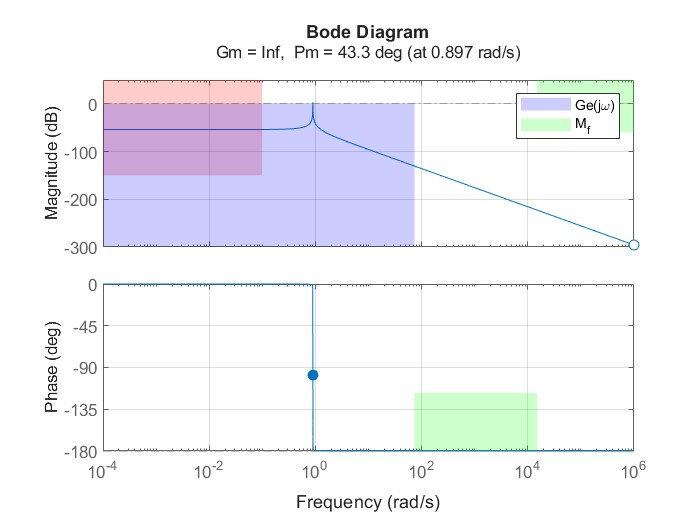
\includegraphics[width=0.7\linewidth]{BodeDiagramWithPatch2025.jpg}
		\caption{Diagramma di Bode della $G(s)$ con le zone proibite in evidenza.}
		\label{fig:patchedG}
	\end{figure}
	
	\newpage
	
	\section{Sintesi del regolatore statico}
	\label{sec:static_regulator}
	
	In questa sezione progettiamo il regolatore statico $R_s(s)$ partendo dalle analisi fatte in sezione~\ref{sec:specifications}: in particolare $L(0) \ge 120$ per la specifica 1 e $L(0) \ge 10^{50/20}$ per la specifica 5; di queste, la seconda è la più stringente. Dato che $L(0) = R(0)G(0)$, sostituendo $G(0) = 0.05$ otteniamo che $R(0) = L(0)/0.05 \ge 6324$ e scegliamo 7000.
	
	Dunque, definiamo la funzione estesa $G_e(s) = R_s(s)G(s)$ e, in Figura \ref{fig:Ge}, mostriamo il suo diagramma di Bode per verificare se e quali zone proibite vengono attraversate.
	
	\begin{figure}[h!]
		\centering
		\includegraphics[width=0.6\linewidth]{BodeGuadagnoStatico.jpg}
		\caption{Diagramma di Bode della $G_e(s)$ con le zone proibite in evidenza.}
		\label{fig:Ge}
	\end{figure}
	
	\newpage
	
	\section{Sintesi del regolatore dinamico}
	
	Dalle analisi fatte in Sezione~\ref{sec:static_regulator}, notiamo di essere nello Scenario di tipo B, in cui tutto l'intervallo di interesse di $\omega_c$ ha fase minore di $-180\degree+M_f = 117.4\degree$.
	Pertanto, per alzare la fase alterando il meno possibile il grafico dell'ampiezza, si prosegue con la progettazione del regolatore dinamico tramite rete anticipatrice del tipo:
	\[
	R_a(s) = \frac{1+\tau s}{1+\alpha\tau s}
	\]
	Si sceglie quindi $\omega_c^\star \ge 73.49$ (specifica 4) e $M_f^\star \ge 62.6$ (specifica 3), e si trovano ampiezza $M^\star$ e fase $\varphi^\star$ risolvendo:
	\begin{subequations}
		\begin{gather}
			|G_e(j\omega_c^\star)|_\dB+20\log M^\star = 0 \\
			M_f^\star = 180\degree + \arg G_e(j\omega_c^\star) + \varphi^\star
		\end{gather}	
	\end{subequations}
	Si trovano infine $\tau$ e $\alpha\tau$ tramite le formule di inversione:
	\begin{subequations}
		\begin{gather}
			\tau = \frac{M^\star-\cos\varphi^\star}{\omega_c^\star\sin\varphi^\star} \\
			\alpha\tau = \frac{\cos\varphi^\star-1/M^\star}{\omega_c^\star\sin\varphi^\star}
		\end{gather}
	\end{subequations}
	
	\begin{figure}[h]
		\centering
		\includegraphics[width=0.7\linewidth]{Ra.jpg}
		\caption{Diagramma di Bode di $R_a(s)G_e(s)$ con le zone proibite in evidenza.}
		\label{fig:Ra}
	\end{figure}
	
	Arriviamo quindi al risultato di Figura \ref{fig:Ra}.
	
	L'unica specifica non rispettata da questo sistema è quella sul disturbo di misura; inseriamo quindi un polo $\omega_p$ alle alte frequenze tale da rispettare la specifica. Otteniamo quindi l'espressione completa del regolatore dinamico:
	\begin{equation}
		R_d(s) = \frac{1}{1+s/\omega_p}\frac{1+\tau s}{1+\alpha\tau s} = \frac{1+0.11s}{(1+s/800)(1+7.25\cdot10^{-4}s)}
	\end{equation}
	
	In Figura \ref{fig:L}, mostriamo il diagramma di Bode della funzione d'anello $L(s) = R_d(s) G_e(s)$
	
	\begin{figure}[h]
		\centering
		\includegraphics[width=\linewidth]{L.jpg}
		\caption{Diagramma di Bode della $L(s)$ con le zone proibite in evidenza.}
		\label{fig:L}
	\end{figure}
	
	\clearpage
	
	\section{Test sul sistema linearizzato}
	
	In questa sezione, testiamo l'efficacia del controllore progettato sul sistema linearizzato in risposta a:
	\begin{itemize}
		\item[a)] il gradino $w(t)=3(t)$
		\item[b)] il disturbo in uscita $d(t)=\sum_{k=1}^{3}3\sin(0.01kt)$
		\item[c)] il disturbo di misura $n(t)=\sum_{k=1}^{3}3\sin(10^5kt)$
	\end{itemize}
	Dopo aver ricavato le funzioni di sensitività $F(s)$ e $S(s)$ si analizza la risposta del sistema al segnale
	al gradino $w(t)$ (in Figura \ref{fig:testlin}), al disturbo $d(t)$ (in Figura \ref{fig:D}) e al disturbo $n(t)$ (in Figura \ref{fig:N}) singolarmente. I disturbi in questi grafici sono attenuati come richiesto da specifiche, per evidenziare che la risposta del sistema è ancora minore.
	
	\begin{figure}[h!]
		\centering
		\begin{subfigure}{0.49\linewidth}
			\centering
			\includegraphics[width=\linewidth]{testlineare.jpg}
			\caption{Risposta al gradino con vincoli di sovraelongazione e tempo di assestamento evidenziati}
			\label{fig:testlin}
		\end{subfigure}
		\hfill
		\begin{subfigure}{0.49\linewidth}
			\includegraphics[width=\linewidth]{D.jpg}
			\caption{Risposta al disturbo $d(t)$}
			\label{fig:D}
		\end{subfigure}
		\\
		\begin{subfigure}{0.49\linewidth}
			\includegraphics[width=\linewidth]{N.jpg}
			\caption{Risposta al disturbo $n(t)$}
			\label{fig:N}
		\end{subfigure}
		\hfill
		\begin{subfigure}{0.49\linewidth}
			\includegraphics[width=\linewidth]{Y.jpg}
			\caption{Risposta complessiva $y(t)$}
			\label{fig:Y}
		\end{subfigure}
	\end{figure}
	
	Mostriamo infine la risposta completa del sistema in Figura \ref{fig:Y}.
	
	
	\clearpage
	
	\section{Test sul sistema non lineare}
	
	In questa sezione, testiamo l'efficacia del controllore progettato sul modello non lineare con Simulink.
	
	Si è realizzato un sistema in retroazione così strutturato:
	
	\begin{figure}[h]
		\centering
		\includegraphics[width=\linewidth]{SistemaNonLinearizzatoB3Immag.png}
		\caption{Schema a blocchi del sistema non lineare}
		\label{fig:SistemaNonLineare}
	\end{figure}
	
	
	\begin{figure}[h]
		\centering
		\includegraphics[width=\linewidth]{SistemaNonLineare.png}
		\caption{Risposta complessiva del sistema non lineare}
		\label{fig:RispostaNonLineare}
	\end{figure}
	Nel caso di test riportato vengono considerate le condizioni iniziali $x_0 = \begin{bmatrix}
		0 \\
		\theta_e
	\end{bmatrix}$
	\newpage
	
	\section{Punti opzionali}
	
	\subsection{Secondo punto}
	Supponendo un riferimento $\theta(t) = \theta_e$, risulta che il sistema converge a $h(x_e,u_e) = \pi\frac{17}{36}$ per delle condizioni iniziali dipendenti solo da $\theta$, e l'unico valore dell'intorno di $\theta_e$ per cui converge a  $h(x_e,u_e)$ risulta essere $\theta=0$.
	
	\subsection{Terzo punto}
	
	Il sistema risulta stabile per ogni valore di $w(t)$; evidenziamo quelli testati.
	
	\begin{figure}[h]
		\centering
		\includegraphics[width=\linewidth]{gradini.png}
		\caption{Valori di $w(t)$ testati.}
		\label{fig:gradini}
	\end{figure}
	
	\section{Conclusioni}
	Dal progetto di controllo di questa macchina motorizzata dotata di disco rotante,
	si può vedere che la risposta del sistema regolato che rappresenta la macchina,
	nella forma non linearizzata, presenta una risposta al gradino complessiva corrispondente, in buona approssimazione, al gradino stesso amplificato.
	La risposta al riferimento $\theta_e$ converge a un valore $\theta(0) + \theta_e$; in particolare, converge a $h(x_e,u_e)$ per $\theta(0) = 0$ e per ogni valore di $\omega(0)$.
	
\end{document}
